\documentclass{article}
\usepackage{iclr2027_conference,times}
\input{math_commands.tex}
\usepackage{amsmath,amssymb,amsthm,booktabs,graphicx,enumitem,xcolor}
\usepackage{hyperref}
\usepackage{url}
\usepackage{microtype}
\newtheorem{proposition}{Proposition}
\newtheorem{remark}{Remark}
\newcommand{\fhat}{\hat{f}}
\newcommand{\code}[1]{\texttt{\small #1}}

\title{Frozen Yet Adaptive: Single-Episode Repair of Vision--Language--Action Policies from Proprioceptive Residuals}
\author{Anonymous authors}

\begin{document}
\maketitle

\begin{abstract}
A vision--language--action (VLA) policy is a large frozen network whose training assumed a
healthy robot. When the execution hardware drifts---a miscalibrated tool frame, a stiff or
weakened joint---the policy is silently wrong, and fine-tuning it is out of reach for most
deployments. We show that the fault can be identified and cancelled \emph{within a single
episode}, from the robot's own motion, by adapting six numbers at the policy's action
interface: a plant model and a sensitivity matrix identified once on healthy data turn the
proprioceptive residual into an estimate of the fault, and a projected, normalised gradient
law drives it to zero. No gradients through the policy, no reward, no reference trajectory,
and no learning across episodes. On four LIBERO suites with a frozen $\pi_{0.5}$, paired
episodes go from $23\%$ to $65\%$ success (exact McNemar $p = 6.1\times10^{-13}$, $n=120$),
with every suite individually significant; across 690 paired episodes spanning additive,
structured, time-varying and multiplicative faults the correction fixes 275 episodes and
breaks 7. The same law repairs two further backbones from two other developers (OpenVLA-OFT,
NVIDIA GR00T N1.7) with the \emph{same} calibration, and, in joint space with a calibration
of their own from a few healthy rollouts, two further manipulators: a bimanual ALOHA and a
humanoid (Fourier GR1 under GR00T N1.5, $4\%\to70\%$, its healthy rate). A tuned integral
baseline without the plant model reaches $35\%$ where the method reaches $95\%$. We state the
two conditions the evidence supports---identifiability, and a repairability criterion
comparing the task's spatial margin against the correction's variation---and the failure
modes that bound the method, including faults invisible to proprioception and a joint lock
that is identified but cannot be cancelled from the action interface.
\end{abstract}

\section{Introduction}

Vision--language--action models map images and a language instruction to robot actions and
are trained on demonstrations collected from a particular robot in a particular state of
repair. Deployed, they are frozen. The robot is not: tool frames drift, calibrations go
stale, joints lose effectiveness. Each changes the map from the policy's action to the
robot's motion, and the policy, which never compares commanded motion with achieved
motion, has no mechanism to notice.

The standard remedies are to fine-tune on faulted data, which requires labelled faults and
the compute to update billions of parameters, or to learn a residual correction offline
against reference rollouts. Both need the fault to be represented in a dataset before it can be corrected---the
closest contemporary method, J-PARC \citep{jparc2026}, trains its calibrator per environment
from faulted rollouts against fault-free references and teacher targets. Neither is
available to a robot that degrades while running.

This paper takes the classical control view. A fault at the action interface is a
disturbance on a plant whose healthy dynamics can be identified once; the disturbance is
observable in the difference between the motion the healthy plant would have produced and
the motion actually measured; and an adaptive law with a handful of parameters can cancel
it online. The question is whether this survives a 3.35B-parameter policy, contact-rich
tasks, and a residual that carries model error as well as the fault. Our contributions:

\begin{enumerate}[leftmargin=1.5em,itemsep=1pt]
\item \textbf{A single-episode repair loop for frozen VLAs} (\S\ref{sec:method}) needing
  only a plant model and a sensitivity matrix identified on healthy data, both properties of
  the robot rather than of the policy or the task. The estimate resets every episode and
  reconverges within a few tens of control steps.
\item \textbf{Evidence at scale, paired} (\S\ref{sec:exp}): four suites, three backbones, three
  manipulators, four fault families, three severities and four time profiles, evaluated
  episode-for-episode against the frozen policy with exact McNemar tests wherever the
  simulator repeats a scene (unpaired Fisher tests on the humanoid benchmark, which
  redraws its scene per reset), a healthy control on every cell, and 690 paired episodes
  in aggregate.
\item \textbf{Two conditions, stated as propositions} (\S\ref{sec:theory}): a constant input
  fault and a constant output bias are not separable within one episode, so the healthy
  bias must be measured outside it; and repair succeeds when the correction's
  within-episode variation fits inside the task's spatial margin, both quantities being
  measurable before any repair attempt. The second predicts every outcome on two further
  manipulators, including the ones continuous adaptation fails.
\item \textbf{The boundary} (\S\ref{sec:fail}): what the method cannot see (sensor and camera
  faults), cannot fix (a policy that fails the task unfaulted), and gets wrong (one healthy
  episode in twenty on one backbone, caused by a sustained phantom).
\end{enumerate}

\section{Related work}
\label{sec:related}

\textbf{VLA policies and their fragility.} $\pi_0$ and $\pi_{0.5}$ generate action chunks
by flow matching from a vision--language backbone; OpenVLA and its OFT variant use an
autoregressive backbone with a regression head. Both are evaluated on LIBERO in a fixed
simulated robot. Robustness to execution faults is not part of the evaluation protocol of
either.

\textbf{Residual calibration of frozen VLAs.} The closest work is J-PARC
\citep{jparc2026}: joint-level physical faults (lock, limited range, friction) on frozen
$\pi_{0.5}$ and OpenVLA-OFT across the same four LIBERO suites, repaired by a residual
calibrator trained \emph{offline}, per environment, from faulted rollouts with fault-free
references and teacher targets ($+6.8$ and $+4.5$ points under joint lock, unpaired). We use
no faulted data, no references and no teacher: the plant is identified once on healthy
motion and the fault online within the episode it occurs in, on paired episodes. Their
faults enter below the controller; ours enter at the action interface, and
\S\ref{sec:joint} tests their class with our law. Closed-loop affine activation editing
\citep{clae2026} steers a frozen policy by editing internal activations against an observed
objective; our correction lives outside the network and needs no access to activations.

\textbf{Adaptive and fault-tolerant control.} Our law is a disturbance observer with
feedforward cancellation, in the MRAC gradient form $\dot\theta = -\Gamma\phi e$, with the
standard robustness modifications (deadzone, normalisation, projection). What is new is
not the law but its target: a frozen generative policy whose command distribution
determines what is identifiable, and a task whose spatial margin determines what is
repairable.

\section{Setting}
\label{sec:setting}

A frozen policy $\pi_\omega$ emits, at 20\,Hz (LIBERO, GR1) or 50\,Hz (ALOHA), an action
chunk from which the controller consumes $a_t\in\mathbb{R}^d$ per step. For LIBERO $a_t$ is
a six-dimensional Cartesian increment plus gripper, executed by an operational-space
controller; for ALOHA it is fourteen and for the GR1 humanoid twenty-nine absolute joint
targets executed by position servos. The measured state $y_t$ is the end-effector
increment (LIBERO) or the joint position (ALOHA, GR1).

A fault corrupts the executed action:
\[
a^{\mathrm{exec}}_t = a_t + f \quad\text{(additive)},\qquad
a^{\mathrm{exec}}_t = \mathrm{diag}(g)\,a_t \quad\text{(multiplicative)},
\]
constant or varying in time. The fault is injected between the policy and the controller.
For LIBERO this models a miscalibrated tool frame or a stale hand--eye calibration; it is
\emph{not} a joint-level actuator fault, which would enter below the controller where the
fault-to-motion map is state dependent (\S\ref{sec:limits}).

The policy never sees $f$. It sees images and the proprioceptive state, and $\pi_{0.5}$-LIBERO
in particular ignores the state input entirely (zeroing it changes the action by exactly
$0.00000$), so a perception-side fault cannot be constructed for it and an action-side fault
cannot be corrected by it.

\section{Method}
\label{sec:method}

\subsection{Plant, residual, and sensitivity}

On healthy rollouts we identify a per-channel FIR plant
\begin{equation}
\hat y_t = \sum_{\ell=0}^{K} h_\ell\, u_{t-\ell} + c, \qquad K = 6,
\end{equation}
where $u_t$ is the command we \emph{believe} we sent (the policy's action plus any
correction we applied). For LIBERO the plant predicts the increment; for ALOHA it predicts
the position, because there the command is an absolute target that a servo tracks and a
target offset lives in the steady-state position error, not in the increment
(\S\ref{sec:aloha}). The residual
\begin{equation}
r_t = y_t - \hat y_t
\end{equation}
is what the healthy plant cannot explain. Because $u_t$ includes the correction and the
world executes $u_t + f$, $r_t \approx M f$ independently of the correction, so the residual
estimates the \emph{total} fault. $M = \partial(\text{motion})/\partial(\text{fault})$ is a
$d\times d$ sensitivity matrix measured once by open-loop replay: a recorded healthy command
sequence is replayed with and without a per-axis probe, and the mean motion difference per
unit probe gives each column. On the LIBERO plant $M$ is diagonal-dominant with
$\mathrm{cond}(M)=3.0$ and is magnitude independent to within $14\%$ between probes of
$0.02$ and $0.05$; on ALOHA $M\approx I$ with $\mathrm{cond}(M)=7.3$; on the GR1 the
arm block is $0.99\,I$ by a direct step response from a held pose (the replay probe is
contaminated on an arm that touches objects during the replay).

\subsection{The adaptive law}
\label{sec:law}

Per control step,
\begin{equation}
\label{eq:law}
e_t = M^{-1} r_t - b,\qquad
\tilde e_t = \frac{e_t\,\mathbb{1}[\|r_t\|>\delta]}{1+\|r_t\|^2/\rho^2},\qquad
\fhat_{t+1} = \Pi_{[-\kappa,\kappa]}\!\big(\fhat_t + \gamma(\tilde e_t - \fhat_t)\big),
\end{equation}
and the next action is sent as $a_t - \fhat_t \odot m$, where $m$ selects the channels to
correct. The terms are the standard robustness modifications and each earned its place by
fixing an observed failure: the deadzone $\delta$ stops plant noise integrating into drift,
the normalisation damps outlier steps (contacts, joint limits), the projection $\kappa$ keeps
the estimate in a physical box, and $b$ is the healthy-plant phantom---the value $\fhat$
settles at with no fault present---measured offline and subtracted, exactly as a sensor is
zeroed before it is trusted (Proposition~\ref{prop:sep} says why it cannot be fitted
within the episode).

\begin{remark}[Constants are ratios of measured scales]
\label{rem:scale}
Every threshold in \eqref{eq:law} is compared against a quantity with a scale: $\delta$
against the residual norm of the healthy plant, $\rho$ against the residual norm under the
fault, $\kappa$ against the expected fault, the excitation gate of \S\ref{sec:gain} against
the regressor's magnitude. Six silent failures in this work came from carrying a constant
tuned on one plant to another---a deadzone larger than the residual it gated, a normaliser
that attenuated every ALOHA update to $6\%$, a normaliser fed the residual of joints the law
was not estimating, a projection bound that coincided with the true fault and was read as a
measurement. The rule that follows is mechanical: print the scale,
then set the constant as a multiple of it, on every new plant.
\end{remark}

The norms in \eqref{eq:law} are taken over the channels being corrected: on the humanoid
the twelve unmodelled hand joints carry three times the arm's residual, and a norm over all
joints attenuated every arm update until the estimate settled at $13\%$ of the fault. The
fixed point of \eqref{eq:law} is attenuated by $1/(1+\|Mf\|^2/\rho^2)$; at the measured
$\|r\|$ on LIBERO this is $5\%$, matching the observed $2\%$ shortfall, and an
innovation-normalised variant ($e_t = M^{-1}(r_t - M\fhat_t)$, unbiased fixed point) was
indistinguishable there ($0.12\sigma$) at twice the variance. We keep \eqref{eq:law} on
LIBERO and ALOHA and use the innovation form on the humanoid, where the fault is three
times the healthy residual and the bias would be $50\%$.

\subsection{Which channels to correct}
\label{sec:channels}

The separation test---the estimate under a fault minus the estimate on matched healthy
episodes---is the only evidence of identification we accept; a raw $\fhat$ carries the plant
phantom and cannot distinguish identification from bias. For the uniform six-axis fault
used across the LIBERO suites, rotation identifies ($+0.049$ against a true $0.050$) and
translation does not (sign-wrong), so the headline correction is restricted to rotation.
That restriction is a property of \emph{that fault}, not of the channel: on a translation-only
fault the same law identifies translation at $79\%$--$106\%$ and repairs it
(\S\ref{sec:severity}). The uniform fault differs because single-axis responses stop superposing at
$\pm0.05$, the signature of a contact or joint limit reached only when all six axes move.

\subsection{Multiplicative faults}
\label{sec:gain}

For a gain fault the regressor follows from the plant rather than being assumed. The world
executes $g\,u$ and the FIR responds to what it is given, so per channel
\begin{equation}
y_i - \hat y_i = \beta_i\,\phi_i,\qquad \phi_i = \hat y_i - c_i,\qquad \beta_i = g_i - 1,
\end{equation}
the regressor being the FIR-weighted command history, and the regression lives in motion
units with no $M^{-1}$. Estimating $\beta_i$ by recursive least squares on channels whose
$|\phi_i|$ clears an excitation gate, the correction is the exact certainty-equivalent
inverse $a_i/(1+\hat\beta_i)$ with $\hat g_i$ projected away from zero. Two facts matter
here. The compensator \emph{inverts} the estimate, so estimation error is amplified by
$1/\hat g^2$---fourfold at $g=0.5$---and accuracy sufficient for an additive fault is not
sufficient for a multiplicative one. And a wrong regressor is not repaired by adding
parameters: regressing on the instantaneous command instead of $\phi_i$ produced a $33\%$
phantom loss of effectiveness on a \emph{healthy} robot, an intercept made it worse, and the
derived regressor shrank the phantom ninefold and took the $x$-channel separation from
$1.4\sigma$ to $18\sigma$.

\section{Two conditions}
\label{sec:theory}

\begin{proposition}[A constant input fault and a constant output bias are not separable]
\label{prop:sep}
Let $y_t = M(a_t + f) + b + \nu_t$ with $M$ square and full rank, and $f,b$ constant over
the episode. For any $b'$, the fault $f' = f + M^{-1}(b - b')$ reproduces every observation
exactly. Only $Mf + b$ is identified.
\end{proposition}
\begin{proof}
$M(a_t+f') + b' = M a_t + Mf + (b - b') + b' = M(a_t + f) + b$.
\end{proof}
\noindent Consequently the healthy phantom $b$ must come from outside the episode (we measure
it on fault-free rollouts), and a fault that switches on mid-episode is \emph{better} posed
than one present from the start: $b$ is identified before onset and $f$ after.

\begin{proposition}[Repairability]
\label{prop:repair}
Let $\mu$ be the task's spatial margin---the largest steady residual offset at the
end-effector under which the healthy policy still succeeds at its healthy rate---and let
$\sigma$ be the within-episode variation of the applied correction. Repair recovers the
healthy rate when the residual stays within $\mu$ for the whole episode, for which
$\sigma < \mu$ is necessary. Both $\mu$ (by a static-correction sweep) and $\sigma$ (from
the estimator's trajectory on one faulted episode) are measurable without knowing the fault
and without a repair trial.
\end{proposition}
\noindent This is an empirical proposition, not a theorem: it states the quantity the data
turned out to depend on. It predicts LIBERO (a reach with centimetres of margin; $\sigma$ of
$0.019$\,cm per step; repair), ALOHA with continuous adaptation ($\mu<0.5$\,cm;
$\sigma = 0.43$\,cm; no repair), ALOHA with the held estimate ($\sigma=0$; repair)
(\S\ref{sec:aloha}), and the GR1 humanoid both ways (\S\ref{sec:gr1}).

\section{Experiments}
\label{sec:exp}

\begin{figure}[t]
\centering

\includegraphics[width=\linewidth]{fig_convergence.pdf}
\caption{The fault estimate within one episode, from zero, on three robots. Left: LIBERO
spatial, $\pi_{0.5}$, uniform $+0.05$ fault, rotation channels (median and interquartile
range over 20 episodes): two reach $0.04$ by step 60, the third $0.024$, all still rising;
at episode end the separation test puts them at $0.047$--$0.049$. Middle: ALOHA
transfer-cube, $\pi_0$, $+0.02$\,rad on the left arm's six joints; the identification
episode settles at $92$--$96\%$ of the offset, then held (\S\ref{sec:aloha}). Right: GR1
humanoid, GR00T N1.5, $+0.10$\,rad on the seven right-arm joints; $90$--$112\%$ within 100
steps, then held (\S\ref{sec:gr1}).}
\label{fig:convergence}
\end{figure}

\subsection{Protocol}

\textbf{Paired design.} Both arms of every cell run the same (task, initial state, seed)
episodes and differ only in whether the correction is applied (the humanoid benchmark
redraws its scene per reset and is the one unpaired comparison, \S\ref{sec:gr1}); Figure~\ref{fig:convergence}
shows what the corrected arm does inside one episode. We report exact McNemar tests
on the discordant pairs; unpaired tests on these data are conservative and, worse, hide the
regression count. \textbf{Controls.} Every cell has a healthy-frozen control on the same
episodes: a null against a ceiling (frozen already near $100\%$) or a floor (frozen near $0$
unfaulted) is not a null, and four cells in this work were avoidable with that control run
first. \textbf{Noise.} $\pi_{0.5}$ samples its action flow; the identical condition scored
$13/20$, $13/20$, $15/20$ on three runs, so $\pm10$ points at $n=20$ is free variation and we
quote intervals. \textbf{Calibration.} Plant and $M$ were identified once on
\code{libero\_spatial} healthy rollouts with $\pi_{0.5}$ driving and are used unchanged for
every LIBERO suite and for OpenVLA-OFT; ALOHA has its own from eight healthy rollouts, the
GR1 from six.

\subsection{Four suites}
\label{sec:headline}

Uniform $+0.05$ offset on all six action dimensions, rotation-only correction
(\S\ref{sec:channels}), $\pi_{0.5}$-LIBERO.

\begin{center}\small
\begin{tabular}{lrrrrrc}
\toprule
suite & $n$ & frozen & corrected & fixed & broken & exact McNemar \\
\midrule
\code{libero\_spatial} & 20 & 8/20 (40\%) & 18/20 (90\%) & 10 & 0 & $0.0020$ \\
\code{libero\_goal}    & 40 & 15/40 (38\%) & 29/40 (72\%) & 15 & 1 & $0.00052$ \\
\code{libero\_object}  & 20 & 5/20 (25\%) & 16/20 (80\%) & 11 & 0 & $0.00098$ \\
\code{libero\_10}      & 40 & 0/40 (0\%) & 15/40 (38\%) & 15 & 0 & $6.1\times10^{-5}$ \\
\midrule
\textbf{pooled} & 120 & \textbf{28/120 (23\%)} & \textbf{78/120 (65\%)} & \textbf{51} & \textbf{1} & $\mathbf{6.1\times10^{-13}}$ \\
\bottomrule
\end{tabular}
\end{center}

Every suite is individually significant. The long-horizon suite goes from a frozen policy
that never succeeds in forty episodes to fifteen recoveries. The single regression is a
\code{goal} episode the frozen policy itself solves three times in four, with an
ordinary-sized correction. \code{libero\_90}, on which the checkpoint was never fine-tuned,
scores $6/20$ unfaulted and is reported as a competence floor of the policy, not a repair
result.

\subsection{Fault families and severity}
\label{sec:severity}
Figure~\ref{fig:map} and the table give the fault-family by magnitude map
(two cells at $n=40$ in Appendix~\ref{app:map40}; constants ablation in Appendix~\ref{app:abl}).

\begin{figure}[t]
\centering
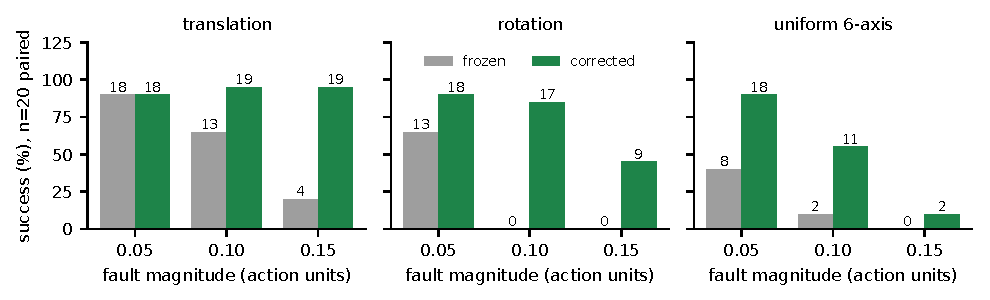
\includegraphics[width=0.92\linewidth]{fig_map.pdf}
\caption{The recoverability map: frozen versus corrected success on LIBERO spatial, $n=20$
paired episodes per cell, correction on the channels each family's separation test
supports (rotation for the rotation and uniform families, translation for translation).
No cell has a regression. Single-family faults degrade gracefully with magnitude; the
uniform fault collapses at $0.15$ because its uncorrected translation component drives the
arm into contacts and limits (\S\ref{sec:fail}). Exact McNemar $p$-values are in the table
below.}
\label{fig:map}
\end{figure}

\begin{center}\small
\begin{tabular}{lccc}
\toprule
fault (\code{libero\_spatial}, $n=20$) & $0.05$ & $0.10$ & $0.15$ \\
\midrule
translation & 18/20 $\to$ 18/20 (ceiling) & 13/20 $\to$ \textbf{19/20} & 4/20 $\to$ \textbf{19/20} \\
rotation    & 13/20 $\to$ 18/20 & 0/20 $\to$ \textbf{17/20} & 0/20 $\to$ \textbf{9/20} \\
uniform 6-axis & 8/20 $\to$ 18/20 & 2/20 $\to$ 11/20 & 0/20 $\to$ 2/20 \\
\bottomrule
\end{tabular}
\end{center}

Zero regressions in every cell. Rotation is where this policy breaks---a rotation fault at
$0.10$ takes it to exactly zero where translation leaves $13/20$---and the correction
recovers $17/20$ from that floor. Single-family faults degrade gracefully with severity; the
uniform fault collapses, and the comparison of the last column isolates why: the rotation
fault and the uniform fault are corrected identically, and adding an \emph{uncorrected}
translation component drops recovery from $45\%$ to $10\%$. The boundary is the plant
leaving the regime where its motion is informative, not the estimator. A structured
mixed-sign fault $[0,0,0,+.06,-.06,+.03]$ the law was never tuned on goes $2/12\to10/12$ with
separation matching truth on every axis.

\textbf{Time-varying faults} (amplitude $0.10$): a ramp to full over 60 steps goes
$12/20\to18/20$ ($p=0.031$); a non-zero-mean oscillation on rotation $13/20\to20/20$
($p=0.016$); an intermittent fault $12/20\to19/20$ ($p=0.039$). The estimator tracks the
waveform poorly---$45$--$79\%$ RMS error, not attributable to lag---and it does not matter:
the correction must be roughly right in direction and scale, not a good tracker, which is
why six numbers updated on CPU suffice. (A zero-mean oscillation averages away and does no
damage; that cell proved nothing and is not counted.)

\textbf{Loss of effectiveness} (\S\ref{sec:gain}): at $g=0.30$, $1/20\to17/20$
($p=3.1\times10^{-5}$) with $\hat\beta = (-0.723,-0.699,-0.717)$ against $-0.700$; at
$g=0.20$, $0/20\to17/20$ ($p=1.5\times10^{-5}$). At $g=0.5$ the frozen policy still scores
$15/20$ and the cell is a ceiling. Rotation gain faults are unidentifiable for this policy:
no recorded step clears the excitation gate on $r_x$ or $r_z$ at any threshold, because the
policy does not rotate the wrist. That is a property of the policy's behaviour, not of the
estimator.

\subsection{Baselines}
\label{sec:baselines}

\textbf{Frozen} and a \textbf{static oracle} correction equal to the true fault bound the
problem. The informative baseline is the one that asks whether the plant model and $M$ earn
their place: \textbf{integral action on the raw motion error}, $\fhat \leftarrow \fhat +
k_i(y_t - a_t)$, swept over five gains across two orders of magnitude. On the $0.15$
translation fault its best setting ($k_i=0.005$) reaches $7/20$ ($35\%$) from a frozen
$3/20$; higher gains fall to $0/20$--$1/20$; ours reaches $19/20$ ($95\%$) on the same
cell. The baseline implicitly assumes achieved motion equals commanded action; the measured plant
DC gain is $0.23$, so with no fault at all its error is $-0.77\,a$---at a command of $0.5$
a phantom of $0.384$ against a real fault of $0.150$, $2.5\times$ the target and opposite in
sign. It must creep to stay stable and saturates when it moves. Predicting $y\approx0.23a$
instead of $y\approx a$ is the whole difference.

\subsection{Faults below the controller}
\label{sec:joint}

Every fault above enters at the action interface. J-PARC's enter in the actuator, where
the fault-to-motion map depends on configuration through the Jacobian. We inject that
class in the MuJoCo model of the LIBERO Panda, below the operational-space controller: a
constant elbow torque (a payload or gravity-compensation error; 5\,N\,m leaks through the
controller as an 8--9\,cm drift over 40 steps, commanded or not), added elbow friction, and
an elbow lock (both invisible while holding, removing 3--10\,cm of commanded motion). An
estimate-only probe identifies each on the translation channels and nowhere else, the lock
at 15--23 healthy-phantom standard deviations. Paired cells, $\pi_{0.5}$,
\code{libero\_spatial}, translation corrected, healthy phantom subtracted:

\begin{center}\small
\begin{tabular}{lrrrrrc}
\toprule
joint fault (elbow) & $n$ & frozen & corrected & fixed & broken & McNemar \\
\midrule
torque bias 5\,N\,m & 40 & 20/40 & \textbf{32/40} & 15 & 3 & $0.0075$ \\
friction $+10$ & 20 & 11/20 & 14/20 & 6 & 3 & $0.51$ \\
friction $+20$ & 20 & 0/20 & \textbf{8/20} & 8 & 0 & $0.0078$ \\
lock $\pm0.05$\,rad & 20 & 0/20 & 0/20 & 0 & 0 & --- \\
\bottomrule
\end{tabular}
\end{center}

The torque bias is repaired, at a cost the Cartesian cells never paid: three regressions
in forty. Its estimate's across-episode spread is 0.075, four times any Cartesian fault's,
because the offset the residual reports is right for the configuration it was measured in
and wrong for the one the arm moves into, and a tracking law follows that with a lag. Heavy
friction, which zeros the policy, is repaired to $40\%$ with no regression; milder friction
is not a claim ($p=0.51$): friction acts only while the joint moves, so an estimate that
was right during a reach pushes the wrong way when the arm pauses to grasp. The lock is
identified, corrected and not repaired: the estimate converges within 30 steps on every
episode, reading the same loss-of-motion signature as the friction cell, and the correction
changes nothing. The difference is physical: friction is a force the controller overcomes
by commanding more, and the correction commands more; a lock removes a degree of freedom,
and no command moves the arm along a direction it can no longer produce. Identifiability
is necessary for repair and not sufficient; the fault must be an input the plant still
responds to. J-PARC's offline residual
reports gains under a lock, consistently: a residual trained on faulted rollouts can learn
a different route through the free joints, and this law cannot.

\subsection{Two further backbones, unchanged calibration}
\label{sec:oft}

OpenVLA-OFT (7B, autoregressive backbone with an L1 action head) and NVIDIA GR00T N1.7
(3B, Cosmos VLM with a flow-matching DiT head, the official LIBERO finetune) are each
served behind the same interface; every script, the plant and $M$ are the $\pi_{0.5}$ ones.

\begin{center}\small
\begin{tabular}{lrrrrc}
\toprule
cell (\code{libero\_spatial}) & frozen & corrected & fixed & broken & McNemar \\
\midrule
healthy control & 20/20 & 19/20 & 0 & 1 & 1.0 \\
rotation $0.10$ & 0/20 & \textbf{11/20} & 11 & 0 & $9.8\times10^{-4}$ \\
translation $0.15$ & 0/20 & \textbf{14/20} & 14 & 0 & $1.2\times10^{-4}$ \\
gain $0.20$ & 0/20 & \textbf{17/20} & 17 & 0 & $1.5\times10^{-5}$ \\
\bottomrule
\end{tabular}
\end{center}

Nothing in the method was $\pi_{0.5}$-specific. OFT is more fragile (frozen $0/20$ on all
three faults), recovers less on rotation ($55\%$ vs $85\%$; its $r_y$ fault is only $23\%$
identified where $\pi_{0.5}$ reached $87$--$100\%$), and the healthy control lost one episode
to the law itself: a sustained phantom at four to ten times the usual size, which a
confidence gate evaluated offline does not remove without delaying genuine repair by one to
two seconds (\S\ref{sec:fail}). The three headline cells also replicate on
\code{libero\_object} with the same calibration ($0/20\to10/20$, $0/20\to15/20$,
$0/20\to19/20$).

GR00T N1.7 is a third developer and a third architecture. Its healthy control is a null
($18/20$ both arms, rotation phantom below $0.005$). With no retuning: rotation $0.10$,
$0/20\to\mathbf{14/20}$ (14 fixed, 0 broken, $p=1.2\times10^{-4}$); translation $0.15$,
$2/20\to\mathbf{15/20}$ (13/0, $p=2.4\times10^{-4}$); gain $0.20$ under the multiplicative
law, $0/20\to\mathbf{19/20}$ (19/0, $p=3.8\times10^{-6}$, $\hat\beta$ within $2\%$ of the
true $-0.80$). Three families, 46 repaired, none broken. The under-identified $r_y$ is the same channel that lags on the other two
backbones: it is a property of the plant and $M$, not of the policy. Across the three
backbones on this cell, 42 of 60 paired episodes are repaired and none is broken.

\subsection{A second manipulator, in joint space}
\label{sec:aloha}

Bimanual ALOHA in \code{gym\_aloha} driven by $\pi_0$: fourteen absolute joint targets at
50\,Hz, transfer-cube, 300-step episodes, healthy success $25\%$. The plant is identified on
\emph{position} from eight healthy rollouts ($R^2 = 0.989$--$1.000$ on all joints),
$M\approx I$. A $+0.05$\,rad offset on the six left-arm joints displaces the gripper by
$5.3$\,cm; the frozen policy scores $0/20$ at every severity tested.

\textbf{Identification transfers.} Separation against the healthy control: $85$--$91\%$ of
the fault at $0.05$\,rad, $94$--$106\%$ at $0.02$\,rad, leakage $\le0.007$\,rad onto
uncorrected joints. \textbf{Repair does not, at first.} With continuous adaptation the task
returns $0/20$ at every severity, warm-started or cold, with or without an early-history
defect we found and fixed. The reason is quantitative:

\begin{center}\small
\begin{tabular}{lccc}
\toprule
correction ($0.02$\,rad fault, $n=20$) & within-episode variation & mean residual & success \\
\midrule
none (frozen) & --- & 2.12\,cm & 0/20 \\
adaptive, updating throughout & 0.43\,cm & 0.17\,cm & 0/20 \\
$0.019$\,rad ($95\%$) applied frozen & 0 & 0.11\,cm & \textbf{5/20} \\
\textbf{adapt episode 0, then hold}, $n=40$ & \textbf{0} & 0.12\,cm & \textbf{15/40} ($p=6.1\times10^{-5}$, 0 broken) \\
healthy, no fault, $n=40$ (law running: 14/40, $p=0.58$) & --- & --- & 17/40 \\
\bottomrule
\end{tabular}
\end{center}

A static-correction sweep puts the task's margin under $0.5$\,cm: a $90\%$ correction held
for the whole episode restores nothing, $100\%$ restores the healthy rate. The updating law
reaches a mean residual well inside that margin and still fails, because its correction
moves by $0.43$\,cm within an episode---the whole margin---on an arm that is precise from
step one. The same number, applied stationary, repairs. \emph{Identify, then hold}---adapt during one
sacrificial episode, hold the estimate thereafter, the cost of a calibration
procedure--- recovers $15/40$ from a frozen zero (held estimate $0.019$--$0.020$\,rad, $95$--$101\%$),
indistinguishable from the healthy arm's $17/40$ on the same seeds ($p=0.75$), while the law
on a healthy arm holds a phantom below $0.001$\,rad and changes nothing. This is
Proposition~\ref{prop:repair}, invisible on LIBERO because a Cartesian reach tolerates
centimetres of jitter.

\subsection{A humanoid}
\label{sec:gr1}
Fourier GR1 upper body (two 7-joint arms, two 6-joint dexterous hands, a waist; 29
absolute joint targets at 20\,Hz) in NVIDIA's RoboCasa GR1 simulator, driven zero-shot by
GR00T N1.5, for which GR1 is a pretrained embodiment. Plant from six healthy
episodes ($R^2\ge0.998$ on the arm), $M$ by direct step response ($0.99\,I$ on the arm
block; the replay probe of \S\ref{sec:aloha} is contaminated on an arm in contact),
constants from the measured residual. A $+0.10$\,rad offset on the working arm zeros the
policy on the plate-to-plate task. The simulator randomises the scene at every reset, so
the arms here are \emph{unpaired}: thirty corrected episodes per scheme against frozen and
healthy arms pooled over 90 episodes each, Fisher exact tests.

\begin{center}\small
\begin{tabular}{lrrrcc}
\toprule
scheme & healthy & frozen & corrected & $p$ vs frozen & $p$ vs healthy \\
\midrule
continuous adaptation & 64/90 & 4/90 & 8/30 & $0.0016$ & $2.3\times10^{-4}$ \\
identify episode 0, then hold & 64/90 & 4/90 & \textbf{21/30} & $8.9\times10^{-13}$ & $1$ \\
\bottomrule
\end{tabular}
\end{center}

Held, the estimate ($83$--$118\%$ of the fault per joint) takes the humanoid from $4\%$ to
its healthy rate, and on a healthy arm the law holds a phantom of at most $0.012$\,rad (one joint; under
$0.006$ on the rest) and changes nothing ($19/30$ against $18/30$); updating, the same estimate reaches a third of it, above frozen and
significantly below healthy. Proposition~\ref{prop:repair} decides the
scheme on the third manipulator as on the second.

\subsection{Hardware}
\label{sec:hardware}
The X2 humanoid protocol (a real actuator-authority fault in 134 logged rollouts, invisible in position, recoverable in effort) is in Appendix~\ref{app:hw}; the paired repair on the robot is pending robot time and is the one result this paper does not yet contain.

\section{What does not work, and what was wrong}
\label{sec:fail}

\textbf{Invisible faults.} A proprioceptive bias and a wrist-camera misalignment both
damage the policy and neither reaches the residual (separation $0.004$ against $0.049$ for
an action fault): the method sees the action interface and nothing upstream of it.

\textbf{A policy that cannot do the task.} \code{libero\_90} fails 14 of 20 sampled tasks
unfaulted. Correcting the fault restores nothing because nothing was lost to it.

\textbf{Harm on a healthy robot.} One OFT episode in twenty was lost to a sustained phantom
acted on. A dwell gate removes most spurious openings but not that one, and every setting
delays real repair; separating it needs information the estimator does not have.

\textbf{Refuted explanations, kept.} We proposed that identifiability follows from healthy
action statistics (refuted: translation identifies a single-axis fault at $79\%$); that the
plant is nonlinear on translation (refuted: $M$ is magnitude independent to $14\%$;
superposition fails instead); and that translation correction contributes nothing (refuted:
at $0.15$ it takes $20\%\to95\%$). The record keeps each with the measurement that killed it.

\section{Limitations}
\label{sec:limits}

Faults below the controller are repaired only when they remain inputs the plant responds
to: a joint torque bias and heavy joint friction are, a joint lock is not
(\S\ref{sec:joint}), and the torque bias carries a regression rate the Cartesian cells never
showed.
A joint-space law would see the torque bias as the constant it is; the Cartesian residual
sees it through the Jacobian. On hardware a stiffness loss is invisible in position and recoverable in effort, so the
sensor, not the law, is what changes. On tight-margin tasks the deployable scheme is to hold
the estimate after one episode, a weaker claim about online adaptation than the LIBERO one,
stated as such. The policy's stochasticity gives $\pm10$ points at $n=20$;
we mitigated it with pairing and $n=40$ where it mattered, not by more seeds. We give
propositions, not a recovery theorem; a contraction argument on the composite map is the
natural next step and requires assumptions we could not verify on contact-rich tasks. And
every constant in the law is a ratio of a measured scale that must be re-measured on a new
plant---six of our own failures came from not doing so.

\section{Conclusion}

A frozen VLA can be repaired within one episode by six numbers at its action interface,
given a plant model and a sensitivity matrix identified once on healthy data; the evidence is
paired and broad, the calibration transfers across suites, backbones and manipulators, the
two conditions that govern success are measurable in advance, and the failures are named.
The result the paper still owes is the one on a real robot.

\subsection*{AI use statement}
Generative AI (Claude, Anthropic) was used throughout this work as a coding and writing
assistant under the authors' direction: it wrote and edited the experiment scripts, the
analysis code, the running project record from which this paper is built, and this
manuscript's text; the authors set the research questions, chose the experiments, ran or
supervised every run on their own hardware, and reviewed the outputs. All numbers in the
paper are recomputed from stored per-episode outcomes by a stdlib-only script, so no
reported figure rests on model-generated text. Three mechanistic explanations proposed
during the work, some AI-generated, were refuted by our own measurements and are reported
as such (\S\ref{sec:fail}). Related work was verified against the cited preprints. We take
responsibility for the final content of this work, including text, claims and artifacts
produced with the aid of generative AI.

\subsection*{Reproducibility statement}
Every number above is recomputed from stored per-episode outcomes by \code{openpi/mcnemar.py}
with nothing installed; the anonymised repository holds those outcomes, the plant and
sensitivity calibrations, and every script named in the paper. Experiments need openpi at
commit \code{15a9616}, the \code{pi05\_libero} checkpoint, and one GPU. The two-virtualenv
split, the OpenVLA-OFT and ALOHA environments, and the three pins that were not obvious
are in \code{SETUP.md}. The law's constants are stated as ratios of measured scales
(\S\ref{sec:method}), which is what made the calibration transfer across suites and
backbones without retuning.

\bibliography{refs}
\bibliographystyle{iclr2027_conference}

\appendix
\section{Ablation of the law's constants and the calibration size}
\label{app:abl}
Headline cell ($\pi_{0.5}$, \code{libero\_spatial}, uniform $+0.05$, rotation-only
correction), $n=20$ paired per row, one constant changed per row from the reference
($\gamma=0.08$, $\rho=0.15$, deadzone $0.008$, plant fitted on three healthy episodes,
285 steps). Last column: rotation estimate at episode end (last-50-step mean) against a
true $0.05$ on each axis.

\begin{center}\small
\begin{tabular}{lrrrrcl}
\toprule
setting & frozen & corrected & fixed & broken & McNemar & $\hat f_{rx},\hat f_{ry},\hat f_{rz}$ \\
\midrule
reference & 8/20 & \textbf{18/20} & 10 & 0 & $0.0020$ & 0.044, 0.020, 0.044 \\
$\gamma=0.02$ ($\tfrac14\times$) & 8/20 & 17/20 & 9 & 0 & $0.0039$ & 0.036, 0.016, 0.036 \\
$\gamma=0.32$ ($4\times$) & 7/20 & 18/20 & 11 & 0 & $0.00098$ & 0.044, 0.019, 0.044 \\
$\rho=0.05$ ($\tfrac13\times$) & 11/20 & 14/20 & 5 & \textbf{2} & $0.45$ & 0.027, 0.011, 0.027 \\
$\rho=0.50$ ($3\tfrac13\times$) & 8/20 & \textbf{20/20} & 12 & 0 & $0.00049$ & 0.048, 0.022, 0.049 \\
deadzone $0$ & 8/20 & 19/20 & 11 & 0 & $0.00098$ & 0.044, 0.018, 0.044 \\
deadzone $0.03$ ($\approx$ residual scale) & 8/20 & 17/20 & 9 & 0 & $0.0039$ & 0.031, 0.016, 0.032 \\
plant from 1 healthy episode (75 steps) & 10/20 & 17/20 & 8 & 1 & $0.039$ & 0.027, 0.008, 0.044 \\
plant from 2 healthy episodes & 8/20 & 17/20 & 10 & 1 & $0.012$ & 0.045, 0.021, 0.043 \\
\bottomrule
\end{tabular}
\end{center}

The gain is flat across a $16\times$ range: it sets the length of the transient, which at a
quarter of the reference still ends well inside a 220-step episode, and the final estimate is
unchanged. The deadzone is flat until it reaches the residual's own scale, where it eats
signal. The normaliser is the one constant that decides the outcome, in the direction the
law's fixed point $f/(1+|r|^2/\rho^2)$ predicts: $\rho=0.05$ against a measured residual of
$0.034$ puts the estimate at $55\%$ of the fault and the cell becomes a null with two
regressions; $\rho=0.50$ removes the bias and the cell reaches $20/20$. The only setting that
fails is the one chosen below the measured residual scale, which is the content of the
``constants as ratios of measured scales'' rule in \S\ref{sec:method}. One healthy episode,
75 control steps, is enough for the plant: $17/20$ with one rotation axis under-identified
and the other two carrying the repair; two episodes recover the full estimate.

\section{Hardware protocol on the X2 humanoid}
\label{app:hw}
On logs from an X2 humanoid running a learned box-pickup policy, a real actuator-authority
fault (stiffness, damping and feedforward scaled together, $0.1$--$1.3$ across 134
rollouts) is invisible in joint position and recoverable in effort ($r=+0.84$); the plant
is run-varying on load-bearing joints, so calibration must be within-run and in motion; the
detectability floor is $0.5$--$1.3^\circ$ of joint offset. The paired repair experiment on
the robot is pending robot time and is the one result this paper does not yet contain.

\section{Recoverability-map cells at $n=40$}
\label{app:map40}
The two cells of \S\ref{sec:severity} that were significant only at the exact test's floor
or just above it were rerun at $n=40$ (same configuration, initial states 45--48). Rotation
$0.05$: $27/40\to39/40$, 12 fixed, 0 broken, $p=4.9\times10^{-4}$. Translation $0.10$:
$30/40\to38/40$, 9 fixed, 1 broken, $p=0.021$. Every map cell that showed an effect at
$n=20$ is individually significant; uniform $0.15$ is the superposition boundary and is not.

\end{document}
